\section{Nota teórica}
\subsection{Información general del MCU}

El microcontrolador ($\mu C$) utilizado en este laboratorio es el PIC12F675 del fabricante \textit{Microchip}, el cual se trata de un microcontrolador de 8 bits tipo CMOS. 
Consta de una célda FLASH de 1024 palabras para alamacenar la memoria de programa. Posee 4 canales de conversión analógico a digital (ADC), 1 canal de comparador, resistores \textit{pull-up} programables, 4 selecciones de osciladores, y 128 bytes de memoria EEPROM.
El diagrama de pines del $\mu C$ se muestra a contiuación:

\begin{figure}[!h]
    \centering
    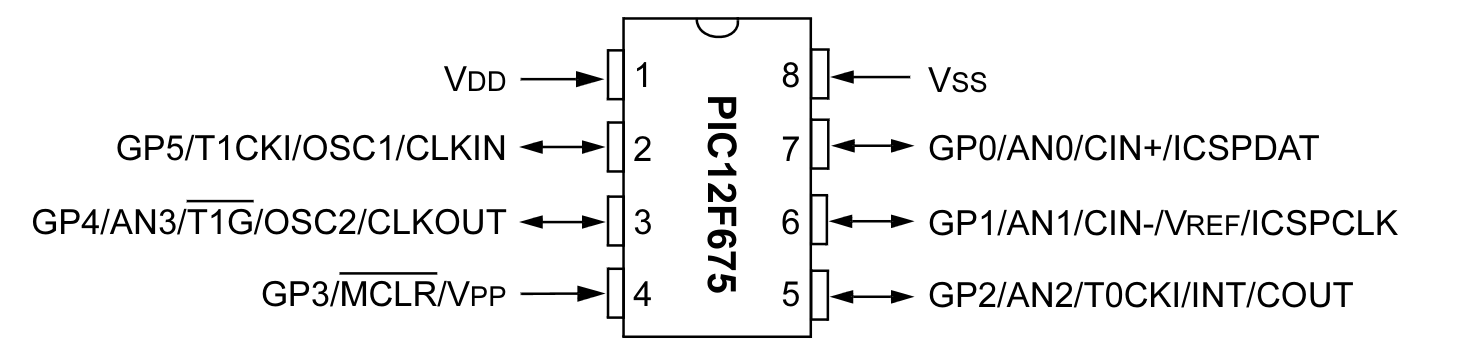
\includegraphics[width = 0.8\linewidth]{imagenes/fig1.png}
    \caption{Diagrama de pines del $\mu C$ PIC12F675}
    \label{fig1}
\end{figure}

Además, este microcontrolador posee una arquitectura RISC de alto rendimiento, la cual consiste de 35 instrucciones y una frecuencia de operación de \SI{20}{MHz}. 
Este microcontrolador es fácilmente adaptable para aplicaciones automotrices, industriales, y para aplicaciones de menor escala gracias a su reprogramibilidad. 
Sus características eléctricas se resumen en la siguiente tabla:

\begin{figure}[!h]
    \centering
    \begin{tabular}{lr}
          \toprule
          Característica eléctrica& Valor máximo absoluto\\ 
          \midrule
          Temperatura ambiente mientras esté polarizado & \SI{-40}{\degreeCelsius} a \SI{+125}{\degreeCelsius}\\
          Temperatura de almacenamiento & \SI{-65}{\degreeCelsius} a \SI{+150}{\degreeCelsius}\\
          Voltaje en $V_{DD}$ con respecto a $V_{SS}$ & \SI{-0.3}{V} a \SI{+6.5}{V}\\
          Voltaje en $\overline{MCLR}$ con respecto a $V_{SS}$ & \SI{-0.3}{V} a \SI{+13.5}{V}\\
          Voltaje en todos los otros pines con respecto a $V _{SS}$ & \SI{-0.3}{V} a $(V _{DD} + \SI{0.3}{V})$\\
          Potencia total disipada & \SI{800}{mW}\\
          Corriente máxima saliente en el pin $V _{SS}$ & \SI{300}{mA}\\
          Corriente máxima entrante en el pin $V _{DD}$ & \SI{250}{mA}\\
          Corriente clamp de entrada $I _{IK}$ $(V _{I}<0\ \text{o}\ V _{I}>V _{DD})$ & $\pm \SI{20}{mA}$\\
          Corriente clamp de salida $I _{OK}$ $(V _{O}<0\ \text{o}\ V _{O}>V _{DD})$ & $\pm \SI{20}{mA}$\\
          Corriente máxima de salida sourced por cualquier pin I/O & \SI{25}{mA}\\
          Corriente máxima de salida sinked por cualquier pin I/O & \SI{25}{mA}\\
          Corriente máxima sunked por todos los pines GPIO & \SI{125}{mA}\\
          Corriente máxima sourced por todos los pines GPIO & \SI{125}{mA}\\
          \bottomrule
      \end{tabular}
      \captionof{table}{Especificaciones eléctricas del $\mu C$ PIC12F675}
    \label{t1}
\end{figure}

Con respecto a los periféricos con los cuales cuenta el PIC12F675, posee 6 pines I/O, un módulo de conversión analógico a digital con una resolución de 10 bits con canales programables, un módulo de comparador analógico programable, 2 timers, Timer0 de 8 bits y Timer1 de 16 bits con prescaler programables, y por último, posee la habilidad de ser programado después de que el $\mu C$ haya sido instalado dentro de un sistema completo (ICSP™, In-Circuit Serial Programming™).

El diagrama de bloques de la estructura interna del PIC12F675 se muestra a continuación:
\vfill
\begin{figure}[!h]
    \centering
    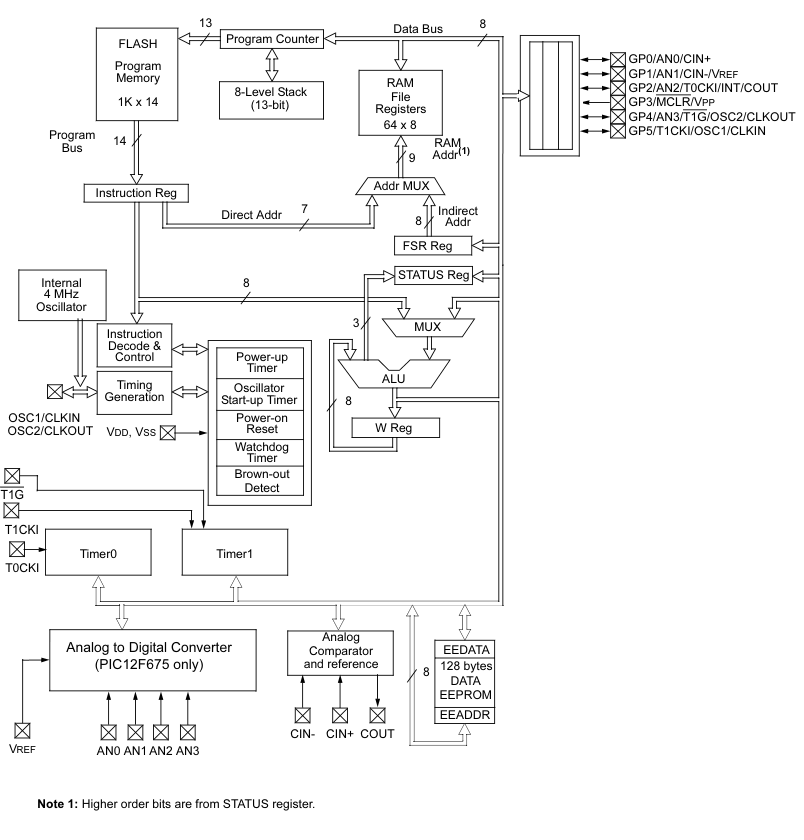
\includegraphics[width = \linewidth]{imagenes/fig2.png}
    \caption{Diagrama de bloques del $\mu C$ PIC12F675}
    \label{fig2}
\end{figure}
\vfill
\newpage
\subsection{Periféricos}

Se manipularon los siguientes periféricos en este laboratorio:

\begin{itemize}
    \item Módulo de conversión analógico a digital
    \item Módulo de comparador analógico
    \item Pines I/O
\end{itemize}

A continuación, se da una breve explicación de cada uno de estos.

\subsubsection{Módulo de conversión analógico a digital}

El módulo de conversión analógico a digital permite la conversión ADC de una señal analógico de entrada a un valor con una resolución de 10 bits. 
El $\mu C$ posee 4 canales analógicos de entrada, los cuales se pueden escoger en software para realizar la conversión de la señal analógico en un pin en particular. 

\begin{figure}[!h]
    \centering
    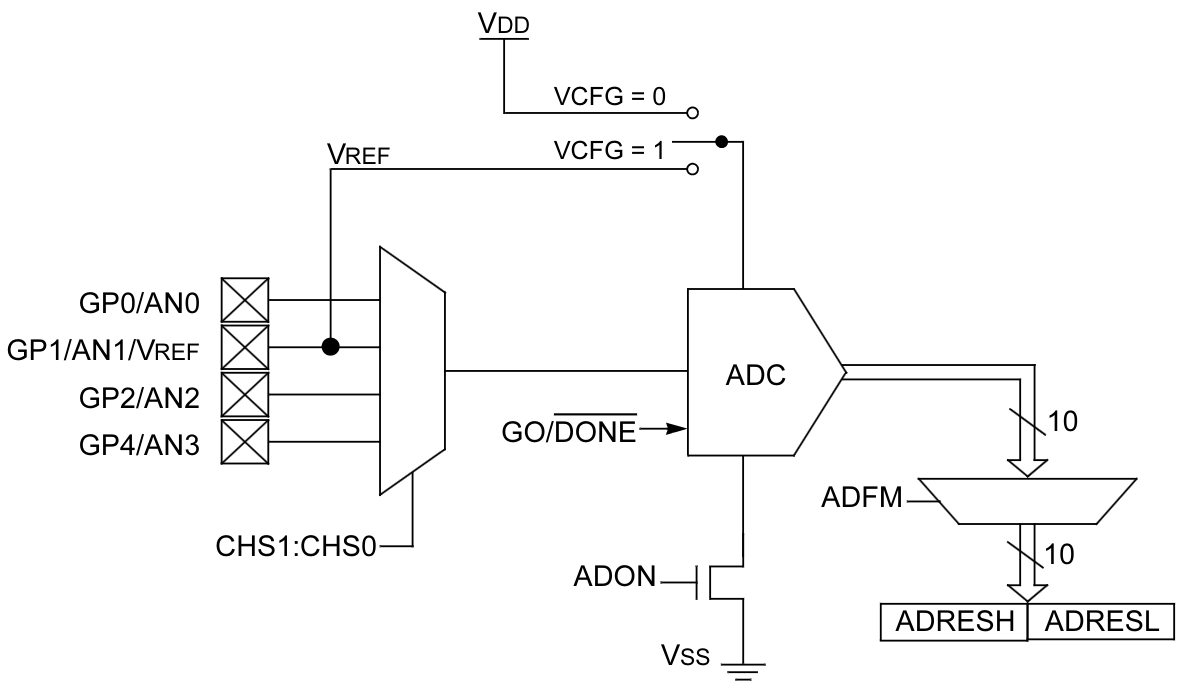
\includegraphics[width = 0.7\linewidth]{imagenes/fig3.png}
    \caption{Diagrama de bloques del módulo de conversión analógico a digital del $\mu C$ PIC12F675}
    \label{fig3}
\end{figure}

El uso y configuración de este módulo se realiza por medio de cuatro registros: 
\begin{itemize}
    \item El registro de configuración ADC \texttt{ADCON0}
    \item El registro de selección analógica \texttt{ANSEL}
    \item Los registros de almacenamiento del resultado de la conversión \texttt{ADRESH} y \texttt{ADRESL}
\end{itemize}

El manejo que se realizó con respecto a estos registro en este laboratorio se explica a detalle en la documentación del código fuente del firmware del controlador, al igual que el valor que se le dio a cada bit.
A continuación, se explica de forma general cada uno de estos registros, haciendo referencia a la funcionalidad de cada bit en los casos respectivos.

\newpage

\paragraph{ADCON0}

En la siguiente tabla, se resume la funcionalidad de cada uno de los bits del registro de configuración ADC \texttt{ADCON0}. 
Esto incluye la abreviación del registro, su funcionalidad, sus cualidades de lectura R(ead) y escritura W(rite), su valor en el \textit{Power on Reset} POR (es decir, el valor del bit después de un reinicio o al momento de energizado), y los posibles valores que los bits pueden tomar.

\begin{figure}[!h]
    \setlength\extrarowheight{3mm}
    \begin{tabular}{clp{3.5cm}cccp{7cm}}
          \toprule
          Bit & Abreviación & Funcionalidad & R & W & POR & \parbox{7cm}{\centering Valores}\\
          \midrule
          0 & ADON    & Habilitación del módulo ADC & \cmark & \cmark & 0& 1 = Módulo ADC habilitado \newline 
                                                                           1 = Módulo ADC deshabilitado\\
                                                                                                        
          1 & GO/$\overline{\text{DONE}}$ & Activación de una conversión ADC & \cmark & \cmark & 0 &
                                                                                          1 = Conversión ADC en progreso. \newline
                                                                                          0 = Conversión ADC finalizado/sin empezar. 
                                                                                              Poner en 1 este bit inicia una conversión ADC. 
                                                                                              Este bit se pone en 0 de forma automática por el hardware al finalizar la conversión\\

          2 -- 3 & CHS$[1:0]$ & Selección del canal analógico & \cmark & \cmark & 0 & 00 = Canal AN0 \newline
                                                                                      01 = Canal AN1 \newline
                                                                                      10 = Canal AN2 \newline
                                                                                      11 = Canal AN3 \\
          5 -- 4 & -- & No implementado & -- & -- & 0 & -- \\
          6 & ADFM & Selección de la justificación del resultado & \cmark & \cmark & 0 &  1 = Justificación derecha \newline
                                                                                          0 = Justificación izquierda\\
          7 & VCFG & Selección de la referencia de voltaje & \cmark & \cmark & 0 & 1 = Voltaje de referencia $V _{ref}$\newline
          0 = Voltaje de referencia $V _{DD}$ \\
          \bottomrule
      \end{tabular}%
      \captionof{table}{Función de los bits del registro \texttt{ADCON0}}
    \label{t2}
\end{figure}

Debido a que el tamaño de los registros de este $\mu C$ es de 8 bits y el resultado de la conversión ADC es de 10 bits, es necesario almacenar el resultado en más de un registro, \texttt{ADRESH} (parte alta) y \texttt{ADRESL} (parte baja). 
Para darle formato al resultado, se escoje por medio del bit ADFM la justificación del resultado; es decir, 8 bits en \texttt{ADRESH} y 2 bits en \texttt{ADRESL} del resultado para justificación izquierda, y viceversa. 
Además de esto, se debe escoger la referencia de tensión $V _{ref}$ o $V _{DD}$ por medio del bit VCFG. 
Para efectos de este laboratorio, se escogió la referencia de voltaje $V _{DD}$ debido a la limitación de pines para crear la cara del dado, y se escogió justificación derecha de forma arbitraria.

\newpage

\paragraph{ANSEL}

De la misma forma que explicó la funcionalidad del registro \texttt{ADCON0}, en la siguiente tabla se resume la funcionalidad de cada uno de los bits del registro de selección analógica \texttt{ANSEL}. 

\begin{figure}[!h]
    \setlength\extrarowheight{3mm}
    \begin{tabular}{clp{3.5cm}cccp{7cm}}
          \toprule
          Bit & Abreviación & Funcionalidad & R & W & POR & \parbox{7cm}{\centering Valores}\\
          \midrule
          0 -- 3 & ANS3:ANS0    & Selección analógica/digital & \cmark & \cmark & 1&  1 = Pin configurrado como entrada analógica \newline 
                                                                                      1 = Pin configurado para que no sea una entrada analógica; I/O digital u otra función\\
                                                                                                        
          4 -- 6 & ADCS$[2:0]$ & Selección de reloj de conversión ADC & \cmark & \cmark & 000 & 000 = FOSC/2 \newline
                                                                                              001 = FOSC/8 \newline
                                                                                              010 = FOSC/32 \newline
                                                                                              X11 = FRC (oscilador interno con frecuencia máxima \SI{500}{kHz})\newline 
                                                                                              100 = FOSC/4  \newline
                                                                                              101 = FOSC/16 \newline
                                                                                              110 = FOSC/64 \\
          7 & -- & No implementado & -- & -- & 0 & --\\
          \bottomrule
      \end{tabular}%
      \captionof{table}{Función de los bits del registro \texttt{ANSEL}}
    \label{t3}
\end{figure}

El tiempo que dura la conversión ADC depende del reloj de conversión ADC que se escoja. 
Aquellos que corresponden a FOSC son divididos por un valor prescaler, permitiendo tener variedad con respecto a los tiempos de conversión ADC.
Para este laboratorio, el tiempo de conversión ADC no es una preocupación, por lo que se escogió FRC. 

\paragraph{ADRESH y ADRESL}

En la siguiente imagen, se resume el comportamiento de los registros de almacenamiento del resultado de la conversión \texttt{ADRESH} y \texttt{ADRESL} de 10 bits para ambos posibles valores de VCFG, en base a la descripción de este bit de \texttt{ADCON0} que se dio anteriormente.

\begin{figure}[!h]
    \centering
    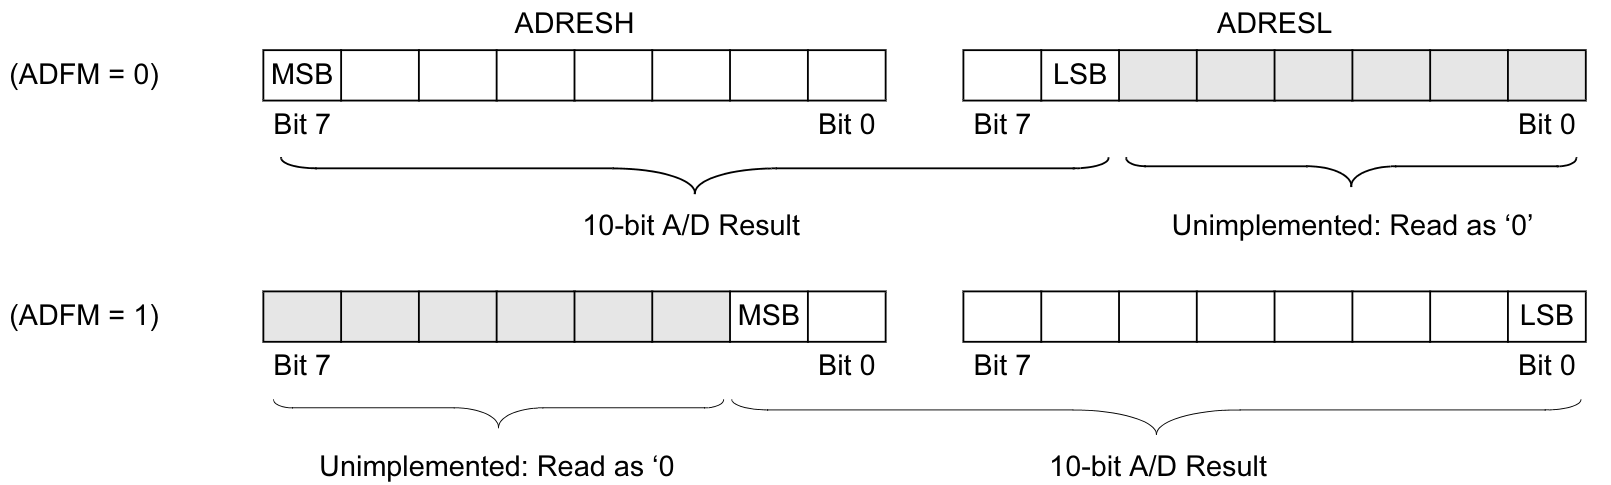
\includegraphics[width = 0.8\linewidth]{imagenes/fig5.png}
    \caption{Registros del resultado ADC de 10 bits \texttt{ADRESH} y \texttt{ADRESL}}
    \label{fig5}
\end{figure}

\newpage

\subsubsection{Módulo de comparador analógico}

El módulo de comparador analógico consta con un comparador programable. 
Es posible configurar por medio de software los pines CIN+ y CIN-- para obtener una lectura alta o baja en las salidas CINV o COUT.

\begin{figure}[!h]
    \centering
    \begin{minipage}{0.4\linewidth}
        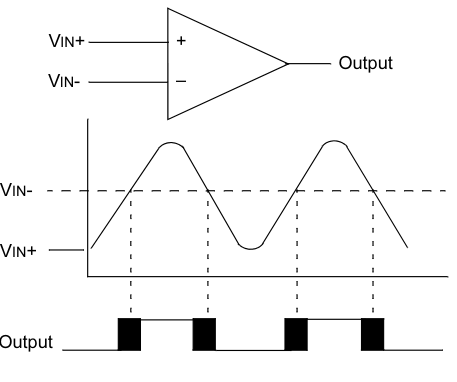
\includegraphics[width = 0.9\linewidth]{imagenes/fig6a.png}
        \caption*{(a): Comparador analógico}
    \end{minipage}%
    \begin{minipage}{0.4\linewidth}
        \begin{tabular}{ccc}
            \toprule
            Condiciones de entrada   & CINV & COUT\\
            \midrule
            $V _{in\,-} > V _{in\,+}$ & 0    & 0\\ 
            $V _{in\,-} < V _{in\,+}$ & 0    & 1\\ 
            $V _{in\,-} > V _{in\,+}$ & 1    & 1\\ 
            $V _{in\,-} < V _{in\,+}$ & 1    & 0\\
            \bottomrule
        \end{tabular}
        \caption*{(b): Salidas del comparador analógico en funcioń de sus entradas}
    \end{minipage}
    \caption{Módulo de comparador analógico}
    \label{fig6}
\end{figure}

Según el valor de los bits CM$[2:0]$ del registro \texttt{ADCON0}, se puede modificar el modo de operación I/O del módulo de comparador analógico. En la siguiente figura, se muestra cada uno de estos modos. 

\begin{figure}[!h]
    \centering
    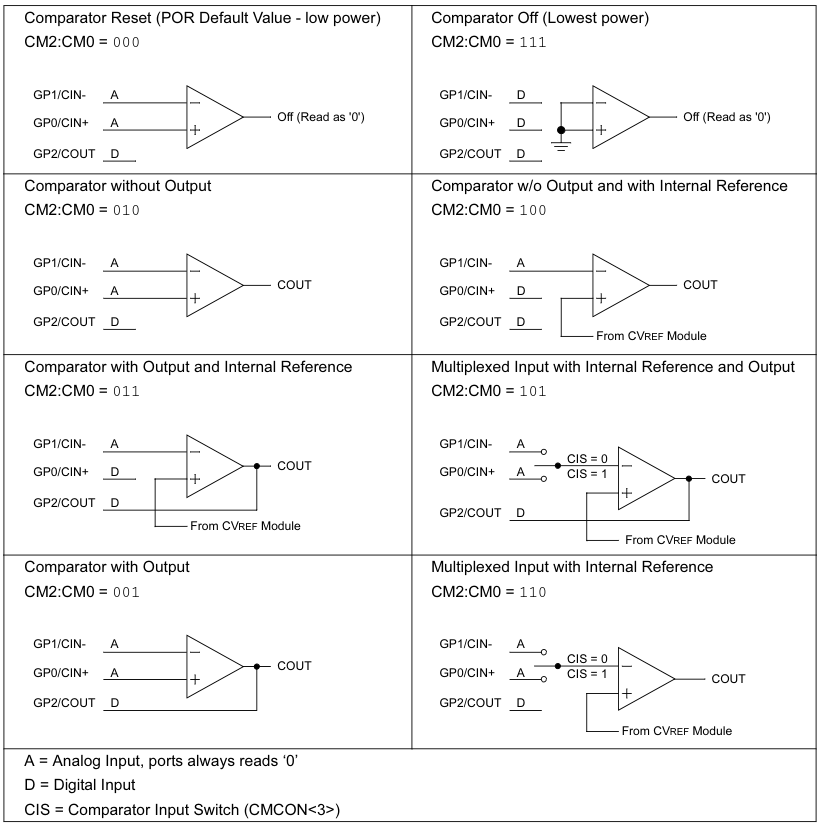
\includegraphics[width = 0.6\linewidth]{imagenes/fig7.png}
    \caption{Modos de operación I/O del módulo de comparador analógico}
    \label{fig7}
\end{figure}

El uso y configuración de este módulo se realiza por medio del registro de control del comparador analógico \texttt{CMCON0}.

\paragraph{CMCON0}

En la siguiente figura, se muestra el registro de control de comparador analógico \texttt{CMCON0}.
A diferencia de los registros mencionados anteriormente, a este registro en particular no se le dará una explicación a fondo debido a que los bits que lo componen no se utilizaron en su totalidad.

\begin{figure}[!h]
    \centering
    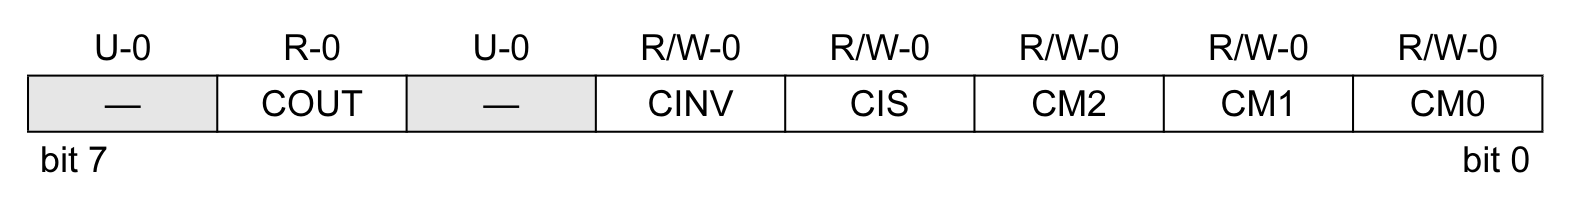
\includegraphics[width = 0.8\linewidth]{imagenes/fig6.png}
    \caption{Registro de control de comparador analógico \texttt{CMCON0}}
    \label{fig66}
\end{figure}

\subsection{Pines I/O}

El $\mu C$ cuenta con 6 pines de propósito general GPIO (\textit{General Purporse Input/Output}).
Los pines correspondiente a GPIOs pueden ser configurados como los mismos, o como un pin asociado a alguno de los periféricos del $\mu C$.  
El uso y configuración de estos pines se realiza por medio de tres registros
\begin{itemize}
    \item El registro \texttt{GPIO}
    \item El registro de tri-estado GPIO \texttt{TRISIO}
    \item El registro de selección analógica \texttt{ANSEL}
\end{itemize}

La única conisderación que debe hacerse con respecto al registro \texttt{ANSEL} es que los bits ANS$[3:0]$ deben ponerse en 0 por software, ya que su valor es 1 en el POR como se puede ver en el Cuadro 3.

\subsubsection{GPIO}

El registro \texttt{GPIO} almacena el valor de un puerto que 

\begin{figure}[!h]
    \setlength\extrarowheight{3mm}
    \begin{tabular}{clp{3cm}cccp{4cm}}
          \toprule
          Bit & Abreviación & Funcionalidad & R & W & POR & \parbox{4cm}{\centering Valores}\\
          \midrule
          0 --  5 & TRISIO$[5:0]$    & Pin I/O de propósito general  & \cmark & \cmark & X & 1 = Puerto del pin es mayor a $V _{IH}$\newline
                                                                                             0 = Puerto del pin es menor a $V _{IL}$\\
          6 -- 7 & -- & No implementado & -- & -- & 0 & --\\ 
          \bottomrule
      \end{tabular}%
      \captionof{table}{Función de los bits del registro \texttt{GPIO}}
      \label{t6}
\end{figure}

\newpage

\subsubsection{TRISIO}
El registro de tri-estado GPIO \texttt{TRISIO} configura los pines GPIO como entradas o salidas digitales.

\begin{figure}[!h]
    \setlength\extrarowheight{3mm}
    \begin{tabular}{clp{3cm}cccp{4cm}}
          \toprule
          Bit & Abreviación & Funcionalidad & R & W & POR & \parbox{4cm}{\centering Valores}\\
          \midrule
          0 -- 2 y 4 -- 5 & TRISIO$[5:4,2:0]$    & Control de tri-estado GPIO  & \cmark & \cmark & X & 1 = Pin GPIO configurado como entrada (en tri-estado)\newline
                                                                                                       0 = Pin GPIO configurado como salida\\
                                                                                     
          3 & TRISIO3 & Control de tri-estado GPIO & \cmark & \xmark & 1 & 1 = Pin GPIO configurado como entrada (en tri-estado)\newline
                                                                           0 = Pin GPIO configurado como salida\\
          6 -- 7 & -- & No implementado & -- & -- & 0 & --\\ 
          \bottomrule
      \end{tabular}%
      \captionof{table}{Función de los bits del registro \texttt{TRISIO}}
    \label{t5}
\end{figure}

La razón del porqué este registro diferencia TRISIO3 es porque GPIO3 se asocia a un pin, el cual también tiene como funcionalidad $ \overline{\text{MCLR}}$, por lo que el pin debe estar en tri-estado para que el MCU ponga GPIO3 = 1 internamente y que el $\mu C$ no inicie con $ \overline{\text{MCLR}} = 0 $.

\subsection{Diseño de circuito}

El diseño del circuito conectado al $\mu C$ se dividió en tres etapas:
\begin{itemize}
    \item Número en la cara del dado
    \item LEDs
    \item Pulsador y manejo de rebotes
\end{itemize}

A continuación, se da una breve explicación de cada etapa, incluyendo la memoria de cálculo para los casos corresponidentes.

\newpage

\subsubsection{Número en la cara del dado}

Para lograr mostrar números del 1 al 6 en la cara del dado, se utilizaron los pines GPIO$[5:4,2:1]$, los cuales se conectaron a LEDs, que a su vez estaban conectados a resistencias para limitar la corriente através de ellos. 
Se optó por conectar 5 de los 6 puertos GPIO cada uno a 2 LEDs a la vez, mientras que el puerto GPIO faltante se conectó al LED central en la cara del dado. 
Dichas conexiones se resumen en la siguiente tabla: 

\begin{figure}[!h]
    \centering
    \begin{tabular}{cc}
        \toprule
        GPIO & Conexiones a la cara del dado\\
        \midrule
        1 & \rotatebox{90}{\Largedice{2}}\\
        2 & \Largetextdice{\(\sbullet[.6] \ \sbullet[.6]\)}\\
        4 & \Largedice{2}\\
        5 & \Largedice{1}\\
        \bottomrule
    \end{tabular}
    \caption{Conexiones entre GPIOs y LEDs que conforman la cara del dado}
    \label{fig8}
\end{figure}

Es posible generar todas las caras del dado deseadas a partir de estas 4 combinaciones. En la documentación del código fuente, se muestra cada combinación.

\subsection{LEDs}

Para diseñar el valor de las resistencias, se consideraron los siguiente circuitos para las conexiones en GPIO$[5:4,2:1]$.

\begin{figure}[!h]
    \centering
    \begin{minipage}{0.4\linewidth}
        \centering
        \begin{circuitikz}[american, scale=0.7, /tikz/circuitikz/bipoles/length=1cm]
            \ctikzset{resistors/scale=0.7, capacitors/scale=0.7, diodes/scale=0.7, inductors/scale=0.7}
            \draw (0,0)to[short, o-] ++(1,0)
                   to[R, l = $R _{5}$] ++(2,0)
                   to[D, fill=red] ++(2,0)
                   node[ground]{};
                  \node[left] at (0,0){\SI{5}{V}};
        \end{circuitikz}
        \caption*{(a): GPIO5}
    \end{minipage}%
    \begin{minipage}{0.4\linewidth}
        \centering
        \begin{circuitikz}[american, scale=0.7, /tikz/circuitikz/bipoles/length=1cm]
            \ctikzset{resistors/scale=0.7, capacitors/scale=0.7, diodes/scale=0.7, inductors/scale=0.7}
            \draw (0,0)to[short, o-] ++(1,0)
            to[R, l = $R _{4,\,1}$] ++(2,0) coordinate (aux)
                   to[D, fill=red] ++(2,0)
                   to[short,-*] ++(0,-2);
            \draw (aux)to[short,*-] ++(0,-2) 
                  to[D, fill=red] ++(2,0)
                  node[ground]{};
                  \node[left] at (0,0){\SI{5}{V}};
        \end{circuitikz}
        \caption*{(b): GPIO$[4:1]$}
    \end{minipage}
    \caption{Circuitos para cada GPIO}
    \label{fig9}
\end{figure}

La luminosidad de cada LED depende de la corriente que pase por cada uno de estos. Este no será un parámetro que se considerará para este diseño, por lo que se tomará $R _{4,\,1} = R_5 = R _{LED}$. 
Considerando una caida de potencial de \SI{2.5}{V} para un LED rojo y considerando una corriente $I _{GPIO} = \SI{10}{mA}$ suministrada por cada pin GPIO utilizado, al aplicar la ley de Ohm a la resistencia $R _{LED}$, se obtiene:

\begin{align*}
    R _{LED} &= \frac{ \SI{5}{V} - \SI{2.5}{V}}{I _{GPIO}}\\
             &= \SI{250}{\ohm}
\end{align*}

Se utilizaron 4 resistencias del valor calculado anteriormente, una para cada GPIO. 
En total, los pines GPIO suministran $ \SI{10}{mA}\times 4 = \SI{40}{mA}$, lo cual se acopla a la máxima corriente sourced por todos los pines GPIO, indicada en las características eléctricas del $\mu C$.
Al consultar la página MicroJPM, no se tienen disponibles resistencias de \SI{250}{\ohm}. 
Por tanto, el valor que se utilizará sería \SI{270}{\ohm}, el cual es el valor de resistencia más cercano por arriba del valor de $R _{LED}$ calculado.
\subsection{Pulsador y manejo de rebotes}

Para el manejo del pulsador que se utilizó para mostrar un número en la cara del dado, se utilizó la siguiente topología:


\begin{figure}[!h]
        \centering
        \begin{circuitikz}[american, scale=0.7, /tikz/circuitikz/bipoles/length=1cm]
            \ctikzset{resistors/scale=0.7, capacitors/scale=0.7, diodes/scale=0.7, inductors/scale=0.7}
            \draw (0,0)to[short, o-] ++(0,-1)
                       to[push button, mirror] ++(0,-2) coordinate(temp)
                       to[R, l=$R _{bounce,\,1}$] coordinate(aux)
                       ++(3,0)
                       to[C, l= $C _{bounce}$, *-] 
                       ++(0,-2)
                       node[ground]{};
                       \draw (aux) to[short, -o] ++(2,0) node[right]{$ \overline{\text{MCLR}}$};
                       \draw (temp)to[R, l_= $R _{bounce,\,2}$, *-] ++(0,-2)
                                   node[ground]{}; 
            \node[above] at (0,0){\SI{5}{V}};
        \end{circuitikz}
    \caption{Circuito para el manejo de rebotes}
    \label{fig10}
\end{figure}

Note que la salida del circuito anterior se conecta a $ \overline{\text{MCLR}}$.
El pulsador despierta al $\mu C$ del reposo para mostrar un número en la cara del dado, minimizando el consumo de potencia.
Para lograr omitir el efecto de los rebotes, se debe diseñar la constante de tiempo $\tau$ para que sea mayor que el tiempo en el cual el botón rebota. 
Considere $\tau = \SI{50}{ms}$. El fabricante recomienda resistencias pull-up de por lo menos \SI{10}{\kohm} en los pines GPIO. Tomando $R _{bounce} = \SI{10}{\kohm}$, para el caso en donde el pulsador es recientemente pulsado se tiene entonces:
\begin{align*}
    \tau_1 &= R _{bounce}C _{bounce}\\
    C _{bounce} &= \frac{\tau_1}{R _{bounce}}\\
                &= \SI{5}{\micro\farad}
\end{align*}

Cuando el botón deja de accionarse, la constante de tiempo cambia ser $\tau_2$. Si $R _{bounce,\,2} = \SI{100}{\ohm}$:
\begin{align*}
    \tau_2 &= \left(R _{bounce,\,1} + R _{bounce,\,2}\right)\cdot C _{bounce}\\
           &= \SI{50.5}{ms}
\end{align*}
Lo cual sigue siendo cercano a los \SI{50}{ms} planteados inicialmente. 

\newpage

\subsection{Circuito total}

En base al diseño del circuito, se construyó el siguiente circuito:

\begin{figure}[!h]
    \centering
    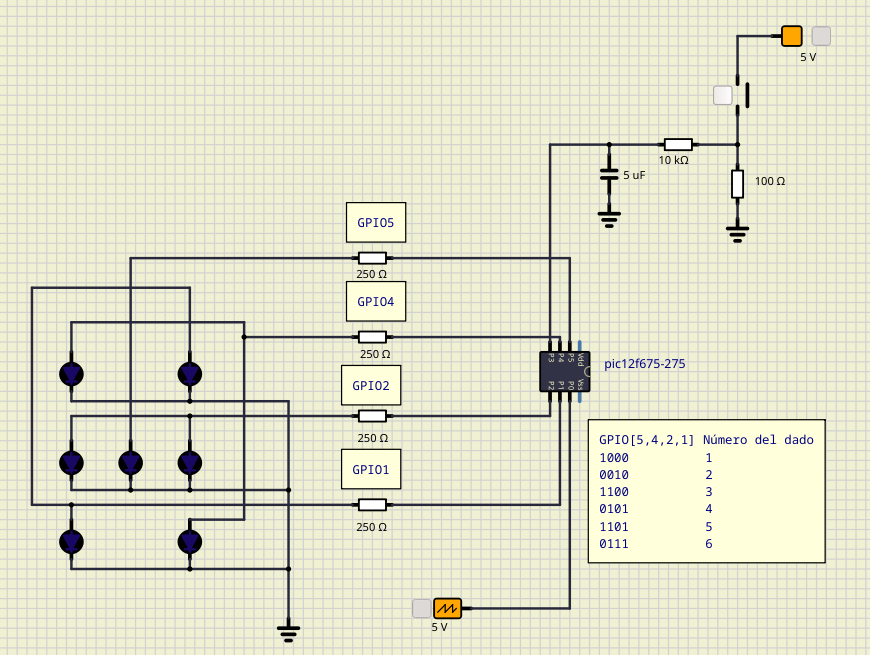
\includegraphics[width = 0.8\linewidth]{imagenes/fig11}
    \caption{Circuito total del simulador de dado}
    \label{fig11}
\end{figure}

Para simular el comportamiento de la tensión en un pin flotante del $\mu C$, se utilizó una fuente de tensión aleatoria en AN0, lo cual es leído por el módulo ADC para generar números aleatorios.

\subsection{Lista de componentes y precios}

A continuación se muestra una lista de todos los componentes utilizados en el diseño del simulador de dado, así como sus precios.

\begin{figure}[!h]
    \centering
    \begin{tabular}{ccccc}
        \toprule
        Componente & Sigla & Cantidad & Valor & Precio\\
        \midrule
        Resistor & $R _{bounce,\,1}$ & 1 & \SI{100}{\ohm} & US\$0.05\\
        Resistor & $R _{bounce,\,2}$ & 1 & \SI{10}{\kohm} & US\$0.06\\
        Resistor & $R _{LED}$ & 4 & \SI{270}{\ohm} & US\$0.20\\
        Capacitor & $C _{bounce}$ & 1 & \SI{5}{\micro\farad}& US\$0.28\\
        Microcontrolador & PIC12F675 & 1 & -- & US\$4.95\\
        \midrule
        \multicolumn{4}{c}{Precio total} & US\$5.54\\
        \bottomrule
    \end{tabular}
    \caption{Conexiones entre GPIOs y LEDs que conforman la cara del dado}
    \label{fig12}
\end{figure}

Los valores listados anteriormente corresponden a componentes encontrados en la página MicroJPM.

\subsection{Conceptos/temas del laboratorio}

Se debe de disponer de una forma de alimentar el $\mu C$. 
Esto depende de la plataforma de hardware en la que se implementará el diseño.
En caso de que fuese una breadboard, bastaría con usar una fuente de tensión DC para obtener \SI{5}{V}, pero si se utilizara una tarjeta perforada para hacer el diseño portable, habría que utilizar baterías y un regulador de tensión para generar la fuente de alimentación.

Además de esto, se debe de contar con un programador para el $\mu C$ para cargar el firmware diseñado. 
Esto es de suma importancia a la hora de contabilizar el precio total del proyecto, ya que estos programadores usualmente no son baratos, y posiblemente dificiles de conseguir.


